%% TITLE	Physiological Fluid Mechanics, Summary 7

%% AUTHOR	BINGHUAN W LI (Dept. Chemical Eng/Bio Eng, Imperial)
%%          PETER Y XIE (Dept. Mech Eng, Stanford)

%% compiled in XeLaTeX with Tex Live version 2023.

%% This work is licensed under a Creative Commons Attribution-NonCommercial 4.0 International License.

\documentclass[a4paper]{article}
\def\NotesType{1}
\def\summaryNo{7}
\def\finalise{1}
%% TITLE	Physiological Fluid Mechanics, configuration

%% DATE		- Nov 19, 2023     create

%% AUTHOR	BINGHUAN W LI (Dept. Chemical Eng/Bio Eng, Imperial)
%%          PETER Y XIE (Dept. Mech Eng, Stanford)

%% compiled in XeLaTeX with Tex Live version 2023.

%% This work is licensed under a Creative Commons Attribution-NonCommercial 4.0 International License.

\usepackage[sfdefault]{arimo}
\usepackage[left=1.5cm, right=1.5cm, top=2cm, bottom=1.5cm]{geometry}
\usepackage{amsmath, amsfonts, amssymb, cancel}
\usepackage{unicode-math}
\setmathfont
    [    Extension = .otf,
         BoldFont = XITSMath-Bold,
    ]{XITSMath-Regular}

% % \DeclareMathSizes{10}{12}{10}{9}

% \usepackage{siunitx}
\usepackage{enumitem}
\usepackage{xcolor}
    \definecolor{linkcolour}{rgb}{0,0.2,0.6}
\usepackage{hyperref}
\hypersetup{
    colorlinks,
    breaklinks,
    urlcolor=linkcolour,
    linkcolor=linkcolour,
    citecolor=black,
    pdfauthor={Li, Binghuan W},
    }
\usepackage{graphicx, float}
\usepackage{framed}
\usepackage[export]{adjustbox}

\usepackage{fancyhdr}
    \pagestyle{fancy}
    \fancyhf{}
    \lhead{\textsc{Physiological Fluid Mechanics Summary \summaryNo}}
    \rhead{page \thepage}

\usepackage{tcolorbox}

\usepackage{tikz, circuitikz}

\usepackage{multicol}
    \setlength{\columnseprule}{1pt}

\usepackage{lscape}

\usepackage{booktabs}

\usepackage{pifont}

\setlength\parindent{0pt}

% put color to \boxed math command
\newcommand*{\boxcolor}{orange}
\makeatletter
\renewcommand{\boxed}[1]{\textcolor{\boxcolor}{%
\tikz[baseline={([yshift=-1ex]current bounding box.center)}] \node [rectangle, minimum width=1ex,rounded corners,draw] {\normalcolor\m@th$\displaystyle#1$};}}
 \makeatother

\begin{document}

\section{Lumped Parameter Modelling}
\paragraph{Resistance, Compliance, and Intertance}
\begin{center}
    \begin{tabular}{ccc}
    \toprule
        Resistance & Compliance & Inertance  \\ [.2em]
    \midrule
        $Q = \Delta p / R$ & $\displaystyle Q = C \frac{\partial p}{\partial t}$ & $\displaystyle p = L \frac{\partial Q}{\partial t}$ \\ [.2em]
    \bottomrule
    \end{tabular}
\end{center}
\begin{itemize}
    \item \textbf{Resistance $R$}: analogous to the electrical resistance which models the dissipation of energy. The mass flow rate $Q$ is analogous to the electrical current (usually denoted by $I$), and the pressure $p$ is analogous to the electrical voltage (usually denoted by $V$).
    \item \textbf{Compliance $C$}: this models the expansion of cardiovascular chambers under pressure, allowing it to store more fluid.
    \item \textbf{Inductor $L$}: this models the inertance of the fluid. When the fluid momentum is substantial, as the pressure on forward-flowing fluid reverses, the fluid will not suddenly reverse its direction, but decelerate over a transient.
\end{itemize}

\paragraph{Solving a Lumped Parameter Network} Consider the example lumped parameter network, \\

\begin{minipage}{0.5\textwidth}
    \begin{center}
    \begin{circuitikz}
    \draw (0,0)node[label={$P_1$}]{} to [resistor, R=$R_1$, i_=$Q_1$, o-o] (3, 0)node[label={$P_2$}]{} to [resistor, R=$R_1$, i_=$Q_2$, o-o] (6,0)node[label={$P_3$}]{};
    \draw (3,0) to [capacitor, C=$C$, i_=$Q_3$, o-] (3, -2)node[ground]{} node [left=3em, below=.5em] {$P_g=0$};
    \end{circuitikz}
\end{center}

\end{minipage}
\hfill
\begin{minipage}{0.5\textwidth}
... which yields a linear system with 4 unknowns ($p_2$, $Q_1$, $Q_2$, $Q_3$) and 4 simultaneous equations:

\begin{equation*}
    \begin{cases}
        p_2 - p_1 = R_1 Q_1, \\[.6em]
        p_3 - p_2 = R_2 Q_2, \\[.6em]
        Q_3 = C (p_2^{(t)} - p_2^{(t-1)})/\Delta t,\\[.6em]
        Q_1 = Q_2 + Q_3.
    \end{cases}
\end{equation*}
\end{minipage}

\vspace{.3cm}
Note that $p_2^{(t-1)}$ denotes the pressure $p_2$ at the previous time step $t-1$; $(p_2^{(t)} - p_2^{(t-1)})/\Delta t$ is an expression of the time derivative in the backward Euler fashion. {\color{gray}(\textit{cf.} electrical capacitor $I = C \cdot \mathrm{d}V/\mathrm{d}t$).}\\

The above linear system can be arranged into a matrix system, $\mathbf{A}\mathbf{x} = \mathbf{b}$,
\[
    \begin{bmatrix}
        1 & -R_1 & 0 & 0 \\
        -1 & 0 & -R_2 & 0 \\
        -1 & 0 & 0 & \frac{\Delta t}{C} \\
        0 & -1 & -1 & -1\\
    \end{bmatrix}
    \begin{bmatrix}
        p_2 \\
        Q_1 \\
        Q_2 \\
        Q_3\\
    \end{bmatrix}
    =
    \begin{bmatrix}
        p_1 \\
        -p_3 \\
        -p_2^{(t-1)} \\
        0
    \end{bmatrix},
\]
and can be easily solved by inversion of the coefficient matrix: $\mathbf{x} = \mathbf{A}^{-1}\mathbf{b}$.
%================================================
\section{Windkessel Models}
\begin{figure}[H]
    \centering
    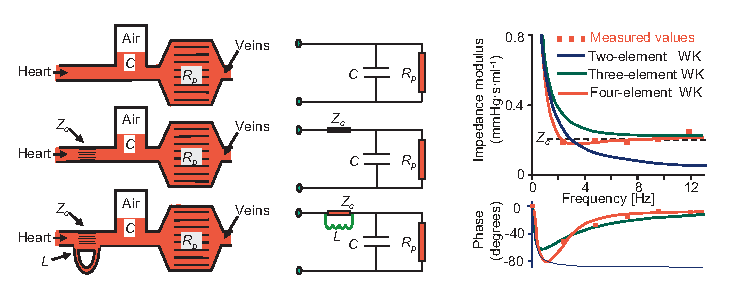
\includegraphics[width=.6\textwidth]{img/winkessel_plot_snapshot.eps}
    \caption{Left: the mechanical equivalence of three Windkessel models; Right: Input impedances of the three Windkessels compared with the measured input impedance. {\color{gray} (Westerhof \textit{et. al})}}
    \label{fig:wk_snapshot}
\end{figure}

\subsubsection*{2-element Windkessel Model}
\begin{minipage}{0.5\textwidth}
\begin{center}
    \begin{circuitikz}
    \draw (0,0) to[vsourcesin, sV=$p(t)$] (0,1) -- (0, 2) -- (2,2)-- (2,1.5) -- (1, 1.5);
    \draw (2, 1.5) -- (3, 1.5);
    \draw (1, 1.5) to [resistor, R=$R$, o-o] (1, -1) -- (2, -1);
    \draw (3, 1.5) to [capacitor, C=$C_{0}$, o-o] (3, -1) -- (2, -1) -- (2, -1.5) -- (0, -1.5) -- (0,0);
    \end{circuitikz}
\end{center}
\end{minipage}
\hfill
\begin{minipage}{0.5\textwidth}
\textbf{Governing Equation:}
\[\frac{\mathrm{d}p(t)}{\mathrm{d}t} + \frac{p(t)}{RC} = \frac{Q_{\rm in}}{C}\]
where $C$ denotes the vessel compliance (elasticity), $R$ denotes the peripheral (distal) resistance.
\end{minipage}

\subsubsection*{3-element Windkessel Model} 
\begin{minipage}{0.5\textwidth}
\begin{center}
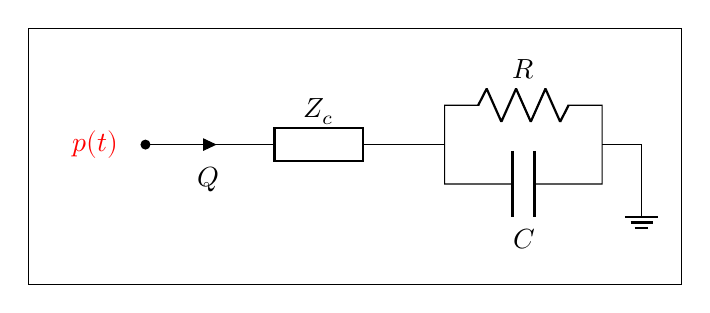
\begin{tikzpicture}
\node[draw, inner sep=8pt] {
    \begin{circuitikz}
    \draw (-.8,0) node[circ,label=left:$\color{red}p(t)$]{} to [short, i_=$Q$](.8,0) to [generic, l=$Z_{c}$](2,0) -- (3,0);
    \draw (3,0) -- (3,0.5) to[resistor, R=$R$] (5,0.5) -- (5,0);
    \draw (3,0) -- (3,-0.5) to[capacitor, l_=$C$] (5,-0.5) -- (5,0);
    \draw (5,0) -- (5.5,0) -- (5.5,-0.5) node[ground]{};
    \end{circuitikz}
};
\end{tikzpicture}
\end{center}
\end{minipage}
\hfill
\begin{minipage}{0.5\textwidth}
\textbf{Governing Equation:}
\[
    \frac{\partial p(t)}{\partial t}
    + \frac{p(t)}{RC} 
    = \frac{Q_{in}}{C} \bigg(1+\frac{Z_{c}}{R}\bigg) 
    + Z_{c} \frac{\partial Q_{\rm in}}{\partial t}
\]
where $Z_{c}$ is the characteristic impedance, $p(t)-p_{\rm distal} = Z_{c}Q_{\rm in}$.
\end{minipage}

\begin{tcolorbox}[title=\textbf{Derivation}, breakable]
    Apply Kirchhoff's Current Law at node $p_{\rm distal}$: $Q_{\rm in} = Q_{R} + Q_{C}$. Moreover, since $p(t)-p_{\rm distal} = Z_{c}Q_{\rm in} \ \Rightarrow \ p_{\rm distal} = p(t) - Z_{c}Q_{\rm in}$.
    \begin{itemize}
        \item Current passes through the resistor $R$:
        \[
            Q_{R} = \frac{p_{\rm distal}}{R} = \frac{p(t) - Z_{c}Q_{\rm in}}{R} = \frac{p(t)}{R} - \frac{Z_{c}Q_{\rm in}}{R}.
        \]
        \item Current passes through the capacitor $C$:
        \[
            Q_{C} = C \frac{\partial p_{\rm distal}}{\partial t} = C \frac{\partial [p(t) - Z_{c}Q_{\rm in}]}{\partial t} = C \frac{\partial p(t)}{\partial t} - CZ_{c}\frac{\partial Q_{\rm in}}{\partial t}.
        \]
    \end{itemize}
    Hence, the total flow $Q_{\rm in}$ is
    \begin{align*}
        Q_{\rm in} 
        & = Q_{R} + Q_{C} \\
        & = \frac{p(t)}{R} - \frac{Z_{c}Q_{\rm in}}{R} + C \frac{\partial p(t)}{\partial t} - CZ_{c}\frac{\partial Q_{\rm in}}{\partial t},
    \end{align*}
    rearrange, we get
    \[
        C\frac{\partial p(t)}{\partial t} 
        + \frac{p(t)}{R} 
        = \bigg( 1+\frac{Z_c}{R} \bigg) Q_{\rm in} + C Z_c \frac{\partial Q_{\rm in}}{\partial t}.
    \]
    Divide both sides of the equation above by $C$, we will get the final governing equation as presented.
\end{tcolorbox}

\subsubsection*{4-element Windkessel Model}
\begin{minipage}{0.5\textwidth}
\begin{center}
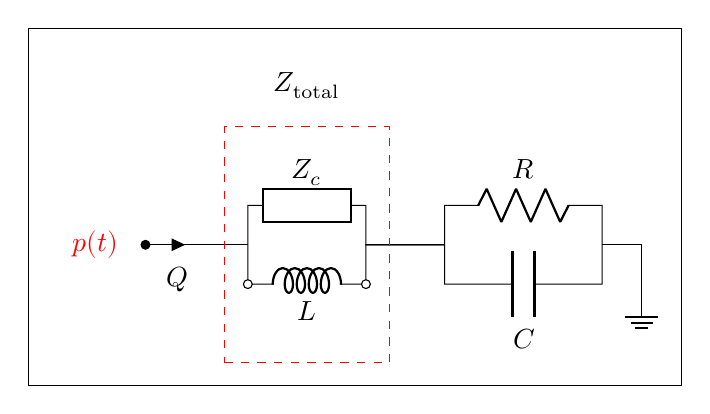
\begin{tikzpicture}
\node[draw, inner sep=8pt] {
    \begin{circuitikz}
    \draw (-.8,0) node[circ,label=left:$\color{red}p(t)$]{} to [short, i_={$Q$}](0,0) -- (.5,0);
    \draw (.5,0) -- (.5,0.5) to [generic, l=$Z_{c}$](2,0.5) -- (2,0) -- (3,0);
    \draw(.5,0) -- (.5,-0.5) to [inductor, l_=$L$, o-o](2,-0.5)-- (2,0) -- (3,0);
    \draw [red, dashed] (.2, -1.5) -- (2.3, -1.5) -- (2.3, 1.5) -- (.2, 1.5) -- cycle;
    \node[above=2pt] at (1.25,1.5) {$Z_{\mathrm{total}}$};
    \draw (3,0) -- (3,0.5) to[resistor, R=$R$] (5,0.5) -- (5,0);
    \draw (3,0) -- (3,-0.5) to[capacitor, l_=$C$] (5,-0.5) -- (5,0);
    \draw (5,0) -- (5.5,0) -- (5.5,-0.5) node[ground]{};
    \end{circuitikz}
};
\end{tikzpicture}
\end{center}
\end{minipage}
\hfill
\begin{minipage}{0.5\textwidth}
\textbf{Governing Equation:}
\[
    \frac{\partial p}{\partial t}
    + \frac{p(t)}{RC} 
    = \frac{Q}{C} \bigg(1+\frac{Z_{\rm{total}}}{R} \bigg)
    + Z_{\rm{total}}\frac{\partial Q}{\partial t}
\]
where $\displaystyle Z_{\rm{total}} = \frac{j\omega L Z_{c}}{j\omega L + Z_{c}}$ is the \rm{total} impedance of the parallel network - the characteristic impedance, $Z_{c}$ and the inductor, $L$. 
\end{minipage}

\begin{tcolorbox}[title=\textbf{Derivation}, breakable]
    Apply Kirchhoff's Current Law at node $p_{\rm distal}$: $Q_{\rm in} = Q_{R} + Q_{C}$. However, we need to express $p_{\rm distal}$ in terms of $p(t)$, hence need to solve the total impedance of the $Z_c$-$L$ parallel network:
    \[
        \frac{1}{Z_{\rm{total}}} = \frac{1}{Z_c} + \frac{1}{j2\pi f L} = \frac{j2\pi f L + Z_c}{j2\pi f L Z_c} 
        \quad \Longrightarrow \quad 
        Z_{\rm{total}} = \frac{j2\pi f L Z_c}{j2\pi f L + Z_c}.
    \]
    Note that sometimes $2\pi f$ is denoted as $\omega$, which is the angular frequency. Now, $p(t)-p_{\rm distal} = Z_{\rm{total}}Q_{\rm in}$. The rest of this derivation follows the same procedure for 3-WK.\\

    \textbf{Necessity of the inductance in 4-WK?} Better capture the frequency characteristics of the flow.
    \begin{itemize}
        \item At the low $f$ range: $2 \pi fL \ll Z_c$, hence $Z_{\rm{total}} \to 0$, which removes the characteristic impedance in the whole circuit;
        
        \item At the high $f$ range: $2 \pi fL \gg Z_c$, hence $Z_{\rm{total}} \to Z_c$.
    \end{itemize}
    This means the inductance has no effect when the flow is steady, providing a zero resistance pathway to the rest of the circuit under steady flow conditions.
\end{tcolorbox}
%=========================================
\section{Moens-Korteweg Model of Pulse Wave Velocity}
\begin{figure}[H]
    \centering
    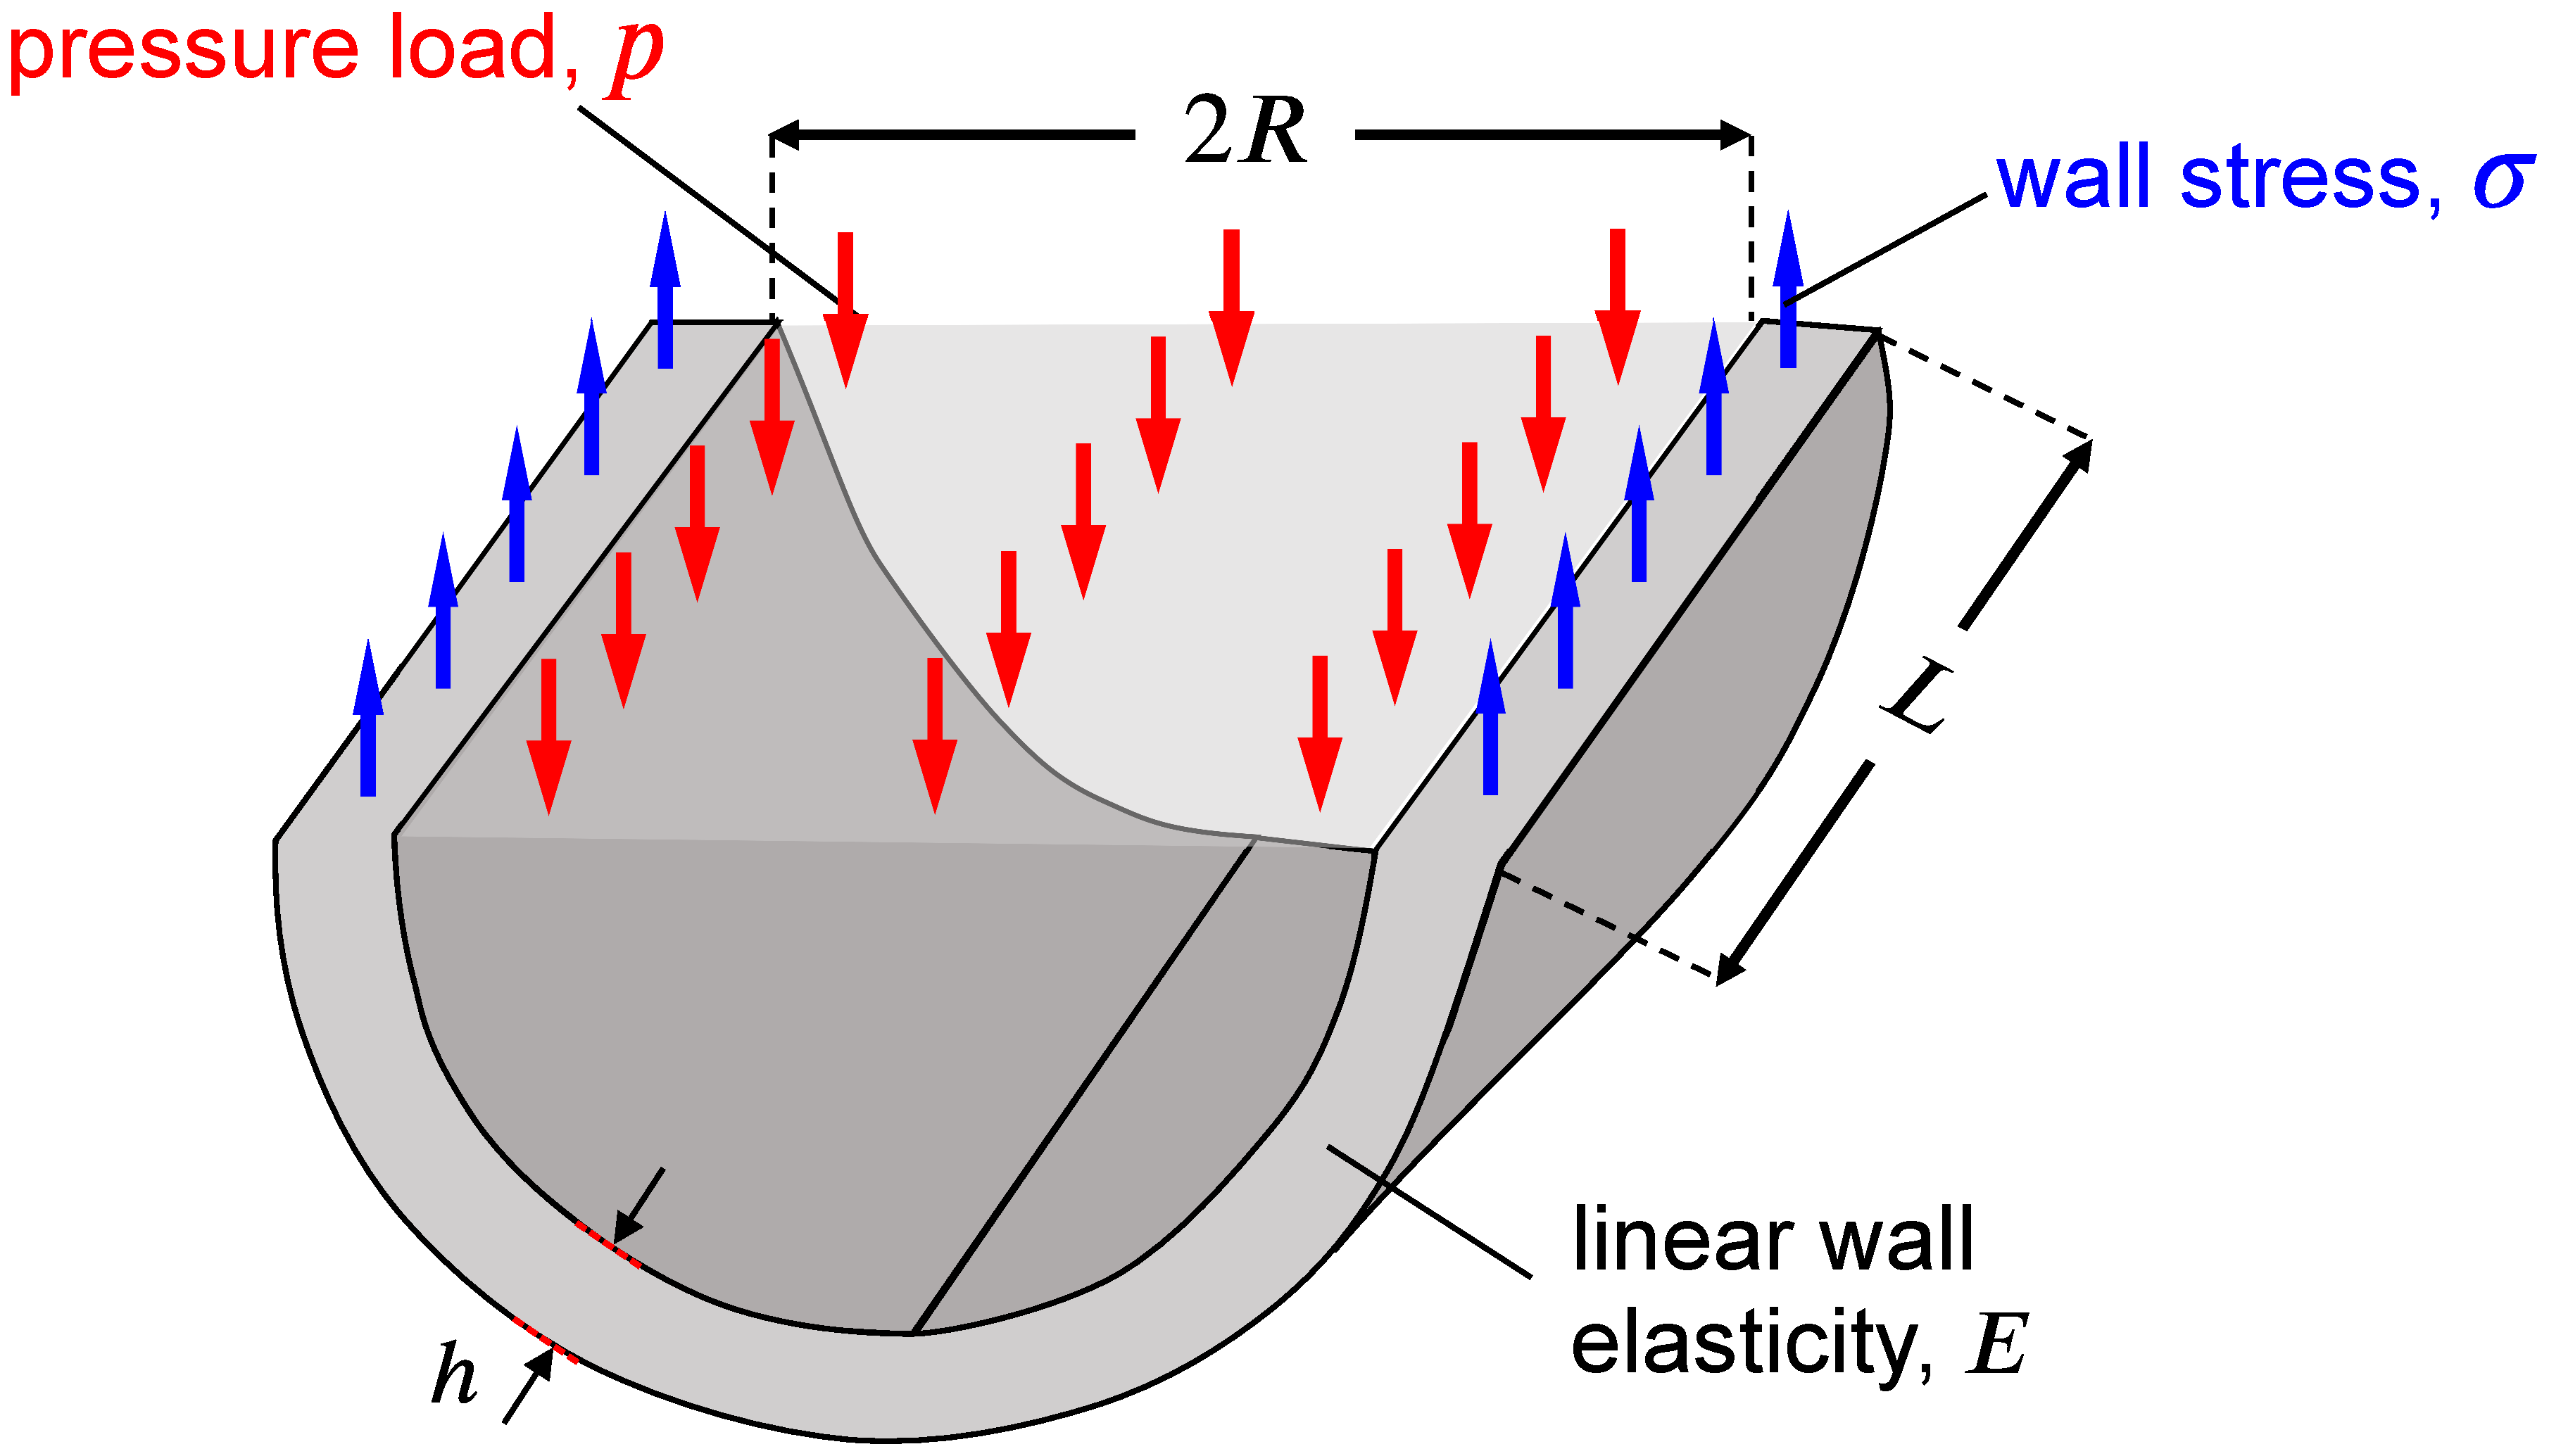
\includegraphics[width=.55\textwidth]{img/Moens-Korteweg.eps}
    \caption{The schematic for the derivation of Moens-Korteweg equation.}
\end{figure}

\paragraph{Equation 1} Assume linear elasticity (fixed Young's modulus, $E$), the stress($\sigma$)-strain($\varepsilon$) relation is 
\[
    \sigma = E \varepsilon = E \frac{\Delta R}{R}
    \quad \text{with} \quad
    \varepsilon = \frac{(2\pi (R+\Delta R) - 2\pi R)}{2\pi R} = \frac{\Delta R}{R}.
\]
Applying Newton's 2\textsuperscript{nd} Law and re-arranging the expression leads to an expression of the pressure,
\begin{align*}
    \begin{split}
        m_{\text{wall}} a_{\text{wall}} 
        & = F_{\text{pressure}} - F_{\text{wall}} \\
        0 & = 2 R L \times P - 2 L h \times \sigma \quad \Rightarrow \quad P = \frac{\sigma h}{R} = \frac{Eh}{R^2} \Delta R.
    \end{split}
\end{align*}
Differentiating $p$ w.r.t. $t$, this leads to \textbf{equation 1},
\[
\boxed{
    \frac{\partial p}{\partial t} = \frac{Eh}{R^2} \frac{\partial \Delta R}{\partial t}
}.
\]

\paragraph{Equation 2}
Integrating the continuity equation over the vascular cross-sectional area 
\begin{align*}
    \frac{1}{r}\frac{\partial ru_{r}}{\partial r} 
    + \cancelto{0, \ \text{axis-symmetrical}}{\frac{1}{r}\frac{\partial u_{\theta}}{\partial \theta}}
    + \frac{\partial u_{z}}{\partial z} = 0
    & \quad \Rightarrow \quad
    \int \bigg( \frac{1}{r}\frac{\partial ru_{r}}{\partial r} + \frac{\partial u_{z}}{\partial z} \bigg) \partial A = 0 \\
    & \quad \Rightarrow \quad
    \int_{r = 0}^{r = R} \bigg( \frac{1}{r}\frac{\partial ru_{r}}{\partial r}\bigg) 2\pi r \partial r + \pi R^2 \frac{\partial \overline{u_{z}}}{\partial z} = 0 \\
    & \quad \Rightarrow \quad
    2 \pi R u_R + \pi R^2 \frac{\partial \overline{u_z}}{\partial z} = 0 .
\end{align*}
Re-arrange leads to the \textbf{equation 2},
\[
\boxed{
    u_r = -\frac{R}{2} \frac{\partial \overline{u_z}}{\partial z}
},
\]
where the notation $\overline{u_z}$ denotes the average $z$-velocity across cross-section.

\paragraph{Equation 3} Assume negligible convective acceleration and no viscous losses, the Navier-Stokes $z$-momentum equation can be simplified as,
\[
    \rho \bigg(\frac{\partial u_{z}}{\partial t} + \cancelto{0}{u_{r} \frac{\partial u_{z}}{\partial r} + \frac{u_{\theta}}{r}\frac{\partial u_{z}}{\partial \theta} + u_{z}\frac{\partial u_{z}}{\partial z}} \bigg) = -\frac{\partial p}{\partial z} + \cancelto{0}{\mu \bigg[ \frac{1}{r}\frac{\partial}{\partial r} \bigg(r \frac{\partial u_{z}}{\partial r}\bigg) + \frac{1}{r^{2}} \frac{\partial^{2} u_{z}}{\partial \theta^{2}} + \frac{\partial^{2} u_{z}}{\partial z^{2}} \bigg]} + \cancelto{0}{\rho f_{z}}
    \quad \Rightarrow \quad 
    \boxed{
    \rho \frac{\partial\overline{u_{z}}}{\partial t} = -\frac{\partial p}{\partial z}
    }.
\]

\paragraph{Derivation of $\mathrm{PVW}$}
First, let $\displaystyle u_r = \frac{\partial \Delta R}{\partial t}$, this equates \textbf{equation 1} and \textbf{equation 2} and leads to \textbf{equation 4}
\[
    \underbrace{u_r = - \frac{R}{2} \frac{\partial \overline{u_{z}}}{\partial z}}_{\text{equation 2}} 
    = \underbrace{\frac{\partial \Delta R}{\partial t} = \frac{R^2}{Eh} \frac{\partial p}{\partial t}}_{\text{equation 1}},
    \quad \Rightarrow \quad
    \underbrace{\frac{\partial \overline{u_{z}}}{\partial z} = -\frac{2R}{Eh} \frac{\partial p}{\partial t}}_{\text{equation 4}}
\]
Next, differentiate \textbf{equation 3} and \textbf{equation 4} w.r.t. $t$,
\begin{align*}
    \rho \frac{\partial \overline{u_z}}{\partial t} = - \frac{\partial p}{\partial z} 
    & \quad \xrightarrow[\text{w.r.t.} \ t]{\text{differentiate}} \quad 
    \rho \frac{\partial^2 \overline{u_z}}{\partial t \partial z} = - \frac{\partial^2 p}{\partial z^2} , \\
    \frac{\partial \overline{u_{z}}}{\partial z}
    = -\frac{2R}{Eh} \frac{\partial p}{\partial t}
    & \quad \xrightarrow[\text{w.r.t.} \ t]{\text{differentiate}} \quad 
    \frac{\partial^2 \overline{u_{z}}}{\partial z \partial t}
    = -\frac{2R}{Eh} \frac{\partial^2 p}{\partial t^2},
\end{align*}
which allows us to equate the R.H.S. as  
\[
    \frac{\partial^2 p}{\partial z^2} = \frac{2 R \rho}{Eh} \frac{\partial^2 p}{\partial t^2}
    \quad \Rightarrow \quad
    \frac{\partial^2 p}{\partial t^2} = \underbrace{\frac{Eh}{2 R \rho}}_{c^2} \frac{\partial^2 p}{\partial z^2},
\]
which can be subsequently re-arranged as the wave equation. Denote the term $\displaystyle \frac{Eh}{2R\rho} = c^2$, for which the term $c$ is the expression of the wave speed of pressure (\textit{a.k.a.} pulse wave velocity, $\mathrm{PVW}$). By definition, $\mathrm{PVW}$ increases with the stiffness of the vessels and decreases with the radius of the vessel.


\vfill
{\small \color{gray}Drafted by B. Li, \today}
% %% TITLE	Physiological Fluid Mechanics, last page

%% DATE		- Nov 19, 2023     create

%% AUTHOR	BINGHUAN W LI (Dept. Chemical Eng/Bio Eng, Imperial)
%%          PETER Y XIE (Dept. Mech Eng, Stanford)

%% compiled in XeLaTeX with Tex Live version 2023.

%% This work is licensed under a Creative Commons Attribution-NonCommercial 4.0 International License.

\newpage
\thispagestyle{empty}
\newgeometry{margin=1.8cm}

\mbox{}
\vfill    
\begin{figure}[H]
    \includegraphics[right]{img/by-nc.eps}
\end{figure}
\textit{This work is licensed under a Creative Commons Attribution-NonCommercial 4.0 International License.}

\end{document}